

The OSI 7-layer model\cite{Zimmermann_1980} describes network communication as a stack of protocols built on top of a \textit{Physical} transport medium such as copper, optical fiber, or radio. On top of the physical layer are the Layer 2 \textit{Data Link} protocols that facilitate reading and writing frames to and from the given physical circuit including source and destination addressing (\textit{Medium Access Control}), and the protocols that encapsulate/de-encapsulate upper layer packets into the frame format suitable for transmission across the medium (\textit{Logical Link Control}). When a datagram from the upper layers is transmitted to a remote system, it is encapsulated into one or more packets at the \textit{Network} layer, the packets are then encapsulated into frames at the Data Link Layer, and the frames are placed onto the physical medium.  When a frame is received at the destination, it is de-encapsulated and the payload is handed up to the Layer 3 \textit{Network} protocol capable of processing the packet. Encapsulation or de-encapsulation occurs between each layer in the OSI model and  adds processing overhead and increased latency to traffic. Layer 2 traffic is not routable, since routing information like IP address is stored in the Layer 3 header. 

% [width=90mm]
\begin{figure}[H]
\centering
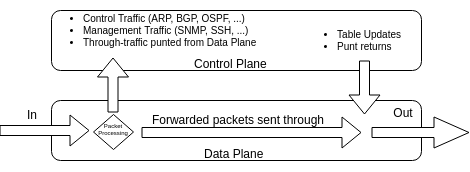
\includegraphics[width=120mm]{img/sgx/sdn/router_flow_2.png}
\caption{Traffic flow between planes}
\label{fig:router_flow}
\end{figure} 

Network device traffic can be partitioned into two planes\cite{Khosravi_Anderson_2003}: the \textit{Forwarding (or Data) Plane} consists of traffic passing through the device while \textit{Control Plane} traffic has the network element as its destination. We consider the \textit{Management Plane} a subset of the \textit{Control Plane}. Forwarding plane components do the heavy lifting in a network device by connecting incoming traffic to the appropriate outgoing port. When the forwarding element can't identify the correct egress port the packet is sent up to the control plane for a routing solution as shown in Figure \ref{fig:router_flow}. The control plane can request and process information about link status and network topology from peers and update forwarding tables in the data plane in response. 

In conventional network equipment the control and data planes are tightly coupled. That is, the components responsible for forwarding packets are physically located along side the components used to make routing and switching decisions about that traffic. How these systems are laid out in practice varies widely by function and vendor. Figure \ref{fig:router_conventional} depicts a notional router. Line cards house the forwarding engine in Application Specific Integrated Circuits (ASICs), Network Processing Units (NPUs), or even software deployed on virtual machines. Incoming traffic is read off the port into a buffer, the packet header is examined to query the Forwarding Information Base for the destination, the packet processor alters the header as needed, and the packet is forwarded out the appropriate egress port. If the traffic is destined for the device (that is, control or management plane) or if the FIB lookup failed, the packets are queued in the receive path buffer for transfer to the routing engine. The routing engine is typically housed on another line card and connected to the forwarding modules through the backplane or switch fabric. Control plane services are hosted by the network OS running on commodity CPUs. The primary purpose of the control plane service suite is to manipulate the forwarding plane lookup tables based on routing and signalling information it receives. It maintains the Routing Information Base (RIB) used to optimize local FIBs and provides the interface for router management and configuration. 

\begin{figure}[H]
\begin{tabular}{p{0.48\textwidth}p{0.47\textwidth}}
\begin{minipage}{.48\textwidth}
\centering
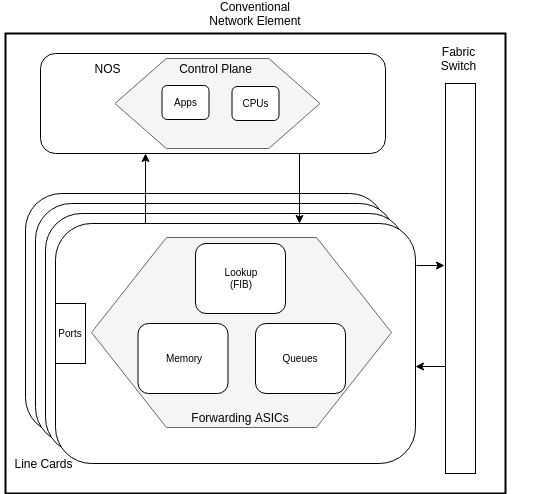
\includegraphics[scale=.4]{img/sgx/sdn/router_conventional.png}
\caption{Conventional Element}
\label{fig:router_conventional}
%\end{figure} 
\end{minipage}
&
\begin{minipage}{.47\textwidth}
\centering
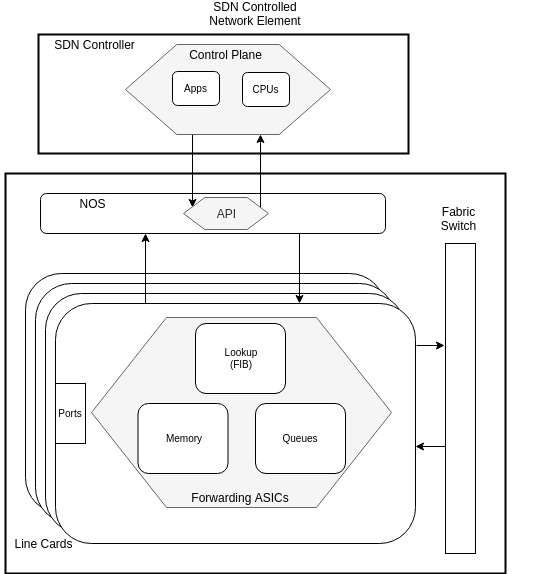
\includegraphics[scale=.4]{img/sgx/sdn/router_sdn.png}
\caption{SDN Controlled Element}
\label{fig:router_sdn}
\end{minipage}
\end{tabular}
\end{figure}

SDN systems decouple the forwarding and control plane elements further, by centralizing controller functionality outside the data plane's enclosure and introducing a southbound interface with which to alter forwarding tables via API. This allows SDN controllers to scale independently of the forwarding elements and receive state information for all network devices it oversees. Since the complex decision logic has been extracted from the forwarding units, the core elements in SDN are simple switches. The result is a control plane that can optimize the forwarding rules it pushes based on global requirements instead of the limited view available to conventional devices. This also results in a potentially larger attack surface and single point of failure. 


Network architectures can be decomposed into tiers based on functionality and proximity to the end users. The \textit{Access} tier is the forward facing attachment point for a user such as the radio tower a mobile device connects with or the set top box that joins a home network to the ISP. The \textit{Provider Edge } provides the services needed to manage traffic between the various access platforms and the provider core. One or more \textit{Aggregation} layers can be added to consolidate provider edge points based on access density requirements. Finally, the \textit{Provider Core} provides hi speed transit between edge nodes. 

\begin{figure}[H]
\centering
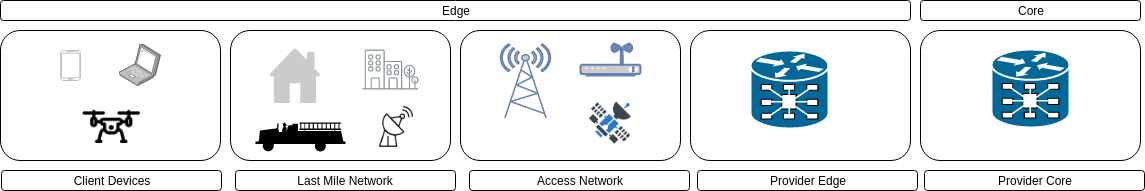
\includegraphics[width=175mm]{img/net_archs/mec_arch_001.png}
\caption{ Network Tiers}
\label{fig:mec_edge}
\end{figure} 